\documentclass[10pt]{beamer}
\usetheme{Marburg}
\graphicspath{{Arquivos/}}
\usepackage[utf8]{inputenc}
\usepackage[french]{babel}
\usepackage[T1]{fontenc}
\usepackage{amsmath}
\usepackage{amsfonts}
\usepackage{amssymb}
\usepackage{graphicx}
\author{Céline Lorentz - Anita Klein - Quentin Dumont - Mariam Grigoryan - Laurène Guidet}
\newcommand{\TT}{Kanban method}
\newcommand{\PI}{I - Introduction}
\newcommand{\PII}{II - Kanban Principles and How it works ?}
\newcommand{\PIII}{III - Advantages}
\newcommand{\PIV}{IV - Disavantages}
\newcommand{\PV}{V - Conclusion}
\title{The Kanban Method}

\begin{document}
    
\begin{frame}

    \maketitle

\end{frame}
\section{\PI} 
\begin{frame}{Introduction}{\PI} 
    \begin{itemize}
        \item 'Kanban' is a Japanese word meaning billboard \textbackslash signboard. 
        \item The kanban method comes from the car industry in Japan.
        \item This method was invented in the late 40's, by Toyota.
        \item The goal was to optimize the car production and be more competitive with American companies.
        \item The main idea is to be able to produce on demand, "just in time".
        \item The software industry began to use it at the beginning of the 21st Century.
        \item It helps you visualize your work and maximize your efficiency.
    \end{itemize}  

\end{frame}
\section{\PII} 
\begin{frame}{Kanban Principles}{\PII}
    \begin{itemize}
        \item 'Kanban' method is a method of a "just-in-time" production 
        \item Wanted quantities.
        \item Limiting production 
        \item Produce to meet the demand
    \end{itemize}  
\quad \quad  \quad \quad \quad \quad 
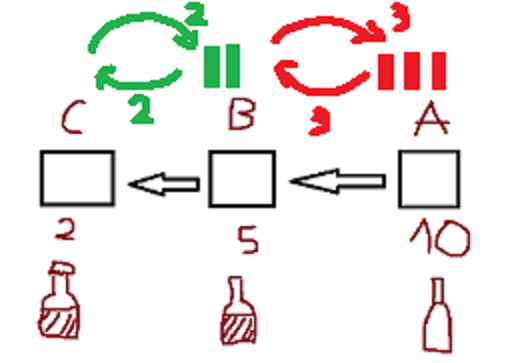
\includegraphics[width=5cm, height=4cm]{kanban.PNG}
    \begin{itemize}
        \item the A's machine products 10 empty bottles per hour
        \item the B's machine fills 5 bottles per hour
        \item The C's machine adds 2 capsules per hour
    \end{itemize}  
\end{frame}

\begin{frame}
    \begin{itemize}
        \item Visualize the workflow
        \item Limiting the number of tasks 
        \item manage the flow
        \item Make policy explicit (unambiguous, direct and clear)
        \item Feedback loops
        \item Improve collaboratively 

    \end{itemize}  
\end{frame}

\begin{frame}{The Concept}{\PII}
    \begin{itemize}
        \item a non-disruptive evolutionary change management system
        \item implementing many minor changes rather than a large one
        \item visualising the workflow
    \end{itemize}
     \begin{figure}
      \centering
   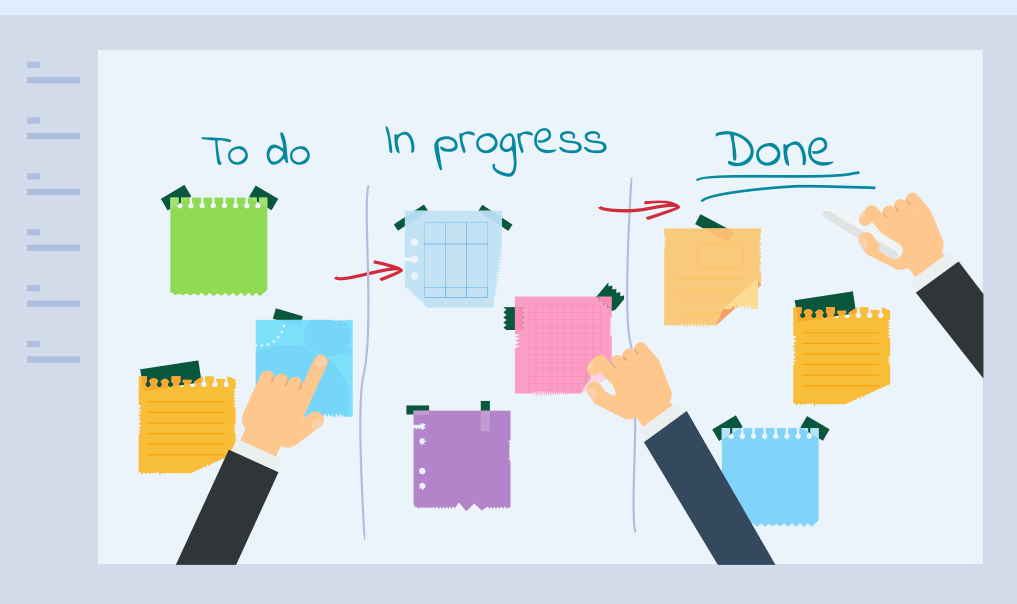
\includegraphics[width=10cm, height=5cm]{ph.png}
      \caption{Task's board}
     \end{figure}
\end{frame}

\section{\PIII} 
\begin{frame}{Advantages}{\PIII}
    \begin{itemize}
        \item avoid waste
        \item do on-demand production
        \item reduction of production costs
        \item quick to set up this method and not expensive
        \item more flexibility in the production
    \end{itemize}

\end{frame}

\section{\PIV} 
\begin{frame}{Disadvantages}{\PIV}
    \begin{itemize}
        \item this method needs a good organization
        \item no anticipation
        \item not adapted for a complex and unrepetitive production
    \end{itemize}
\end{frame}

\section{\PV} 


\begin{frame}{Conclusion}{\PV}
    \begin{itemize}
        \item optimize the production
        \item maximize the efficiency
        \item other methods are better ?
    \end{itemize}
\end{frame}


\begin{frame}{Bibliography}
    \begin{itemize}
        \item https://kanbanize.com/kanban-resources/getting-started/what-is-kanban
        \item https://www.planzone.fr/blog/quest-ce-que-la-methodologie-kanban
        \item https://www.digite.com/kanban/what-is-kanban/#kanban-concept
        \item https://www.amalo-recrutement.fr/blog/logistique-a-flux-tires-et-a-flux-pousses-qu-est-ce-que-c-est/
        \item http://functionalguy.blogspot.com/2007/04/advantages-and-disadvantages-of-kanban.html
        \item https://michel.re/methode-kanban/#19-limites-de-la-méthode-kanban
    \end{itemize}

\end{frame}


\begin{frame}{Methodology}
    \begin{itemize}
        \item First, we split up the work equitably between the five of us.
        \item Then, each of us worked on his part, using Github, in order for everyone to be able to see it.
        \item We had a videoconference call to fix some issues, and finalize this project.
    \end{itemize}
\end{frame}


\end{document}
